\pdfsuppresswarningpagegroup=1

\PassOptionsToPackage{dvipsnames}{xcolor}

\documentclass[
    aspectratio=169,
    %handout,
]{beamer}

\usetheme{Boadilla}
\usecolortheme{seahorse}
\usepackage{pifont}
\usepackage{pgfplots}
\usepackage{svg}
\usepackage{t1enc}
\usepackage{bbding}
\usepackage{enumitem}
\usepackage{fontawesome5}
\usepackage{minted}
\usepackage[hungarian]{babel}
\usepackage[none]{hyphenat}
\usepackage[absolute,overlay]{textpos}
\usepackage{qrcode}
\usepackage{amsfonts}

\pgfplotsset{
    tick label style = {font = {\fontsize{8 pt}{14 pt}\selectfont}},
    every axis label = {font = {\fontsize{8 pt}{14 pt}\selectfont}},
    label style = {font = {\fontsize{10 pt}{20pt}\selectfont}},
    legend style = {font = {\fontsize{6 pt}{10 pt}\selectfont}},
}

\setenumerate{
    label=\arabic*.,
    itemsep=3pt,
    topsep=3pt,
}
  
\setitemize{
    label=\usebeamerfont*{itemize item}%
    \usebeamercolor[fg]{itemize item}
    \usebeamertemplate{itemize item}
}
  
\newlist{logolist}{itemize}{1}
\setlist[logolist,1]{
    label={},
    leftmargin=4em
}

\titlegraphic{
\includegraphics[width=2cm]{elte_cimer_szines}}
\title[HoloDB]{HoloDB: Relációs demóadatok konzisztens on-the-fly generálása\\ deklaratív konfigurációból}
\author[Horváth Dávid]{Horváth Dávid \\ ~ \\ { \footnotesize Témavezető: dr. Vincellér Zoltán, mesteroktató }}
\institute[ELTE-IK]{ELTE Informatikai Kar, Információs Rendszerek Tanszék}
\date{2025}

\newcommand{\slidetitle}[2]{\frametitle{{\small #1 ~ \ding{226} ~ } \normalsize \textbf{#2} }}

\newcommand{\greencheck}{{\color{green!65!black}\ding{51}}}

\newcommand{\textbftt}[1]{{\fontfamily{lmtt}\fontseries{b}\selectfont{#1}}}

\newcommand{\brqr}{
    \begin{textblock*}{2cm}[0,0](\dimexpr\paperwidth-2.5cm\relax,\dimexpr\paperheight-2.5cm\relax)
        \resizebox{2cm}{!}{\qrcode{https://github.com/miniconnect/holodb}}
    \end{textblock*}
}

\newcommand{\best}[1]{{\color{PineGreen}\underline{\textbf{#1}}}}

\newcommand{\bad}[1]{{\color{BrickRed}#1}}

\newcommand{\nodata}{\textcolor{lightgray}{~\footnotesize{N/A}~}}

\begin{document}
\beamertemplatenavigationsymbolsempty

\begin{frame}[plain,noframenumbering]
    \titlepage
\end{frame}

\begin{frame}
    \frametitle{Tartalom}
    \hfill
    \parbox[t]{.95\textwidth}{
        \begin{minipage}[c][0.6\textheight]{\textwidth}
        \tableofcontents
        \end{minipage}
    }
\end{frame}

\section{A probléma: adatbázist akarok, most!}
\def\sectionshorttitle{\arabic{section}. A probléma}

\begin{frame}[fragile]
    \slidetitle{\sectionshorttitle}{Adatbázist akarok, most!}
    
    \begin{minipage}[c]{0.63\textwidth}
        \begin{logolist}
            \setlength\itemsep{1.2em}
            \item[\raisebox{-0.75em}{
\includegraphics[width=2em,height=2em]{image/dbnow-mock}}]
                \begin{minipage}[c]{\linewidth}~~\textbf{mockolás, fejlesztés} \par ~~~~
                    csak legyen ott valami, hogy fusson
                \end{minipage}
            \item[\raisebox{-0.75em}{
\includegraphics[width=2em,height=2em]{image/dbnow-prot}}]
                \begin{minipage}[c]{\linewidth}~~\textbf{tervezés, prototipizálás, kísérletezés} \par ~~~~
                    szeretnénk folyamatosan újragondolni
                \end{minipage}
            \item[\raisebox{-0.75em}{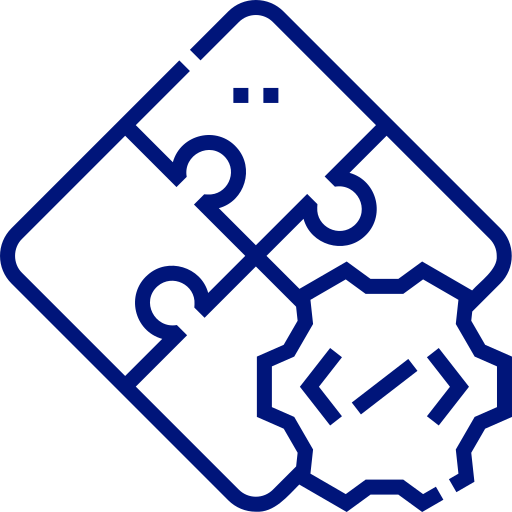
\includegraphics[width=2em,height=2em]{image/dbnow-test}}]
                \begin{minipage}[c]{\linewidth}~~\textbf{integrált tesztelés} \par ~~~~
                    kellenének adatok a tesztfuttatáshoz
                \end{minipage}
            \item[\raisebox{-0.75em}{
\includegraphics[width=2em,height=2em]{image/dbnow-pres}}]
                \begin{minipage}[c]{\linewidth}~~\textbf{bemutatók, koncepciótervek} \par ~~~~
                    értelmes adathalmaz a demózáshoz
                \end{minipage}
            \item[\raisebox{-0.75em}{
\includegraphics[width=2em,height=2em]{image/dbnow-stud}}]
                \begin{minipage}[c]{\linewidth}~~\textbf{oktatás} \par ~~~~
                    egységes homokozó adatbázis tanulóknak
                \end{minipage}
        \end{logolist}
        \pause
    \end{minipage}%
    \hspace*{\fill}%
    \begin{minipage}[c]{0.35\textwidth}
        \centering
        
        \includegraphics[width=\textwidth]{diagram/database-tasks-compressed}
    \end{minipage}%
    \hspace*{\fill}%
\end{frame}

\begin{frame}[fragile]
    \slidetitle{\sectionshorttitle}{A szokásos megközelítések}
    
    \begin{minipage}[c]{0.58\textwidth}
        \begin{logolist}
            \setlength\itemsep{2em}
            \Large
            \item[\raisebox{-0.4em}{\includesvg[width=1.25em]{image/solution-copy}}]
                    ~produkciós adatbázis másolása
            \item[\raisebox{-0.4em}{\includesvg[width=1.25em]{image/solution-anonymize}}]
                    ~anonimizálás
            \item[\raisebox{-0.4em}{\includesvg[width=1.25em]{image/solution-generate}}]
                    ~adatgenerálás
            \item[\raisebox{-0.4em}{\includesvg[width=1.25em]{image/solution-mock}}]
                    ~lekérdezések ad hoc mockolása
        \end{logolist}
        \pause
    \end{minipage}%
    \hspace*{\fill}%
    \begin{minipage}[c]{0.35\textwidth}
        \centering
        
        \begin{minipage}[t]{0.48\textwidth}
            \centering
            
            
\includegraphics[width=0.45\textwidth, frame]{image/mostly-ai}\par
            \textbf{MOSTLY AI}
            
            \vspace{5pt}
            
            
\includegraphics[width=0.45\textwidth, frame]{image/tonic}\par
            \textbf{Tonic}
        \end{minipage}%
        \hspace*{\fill}%
        \begin{minipage}[t]{0.48\textwidth}
            \centering
            
            
\includegraphics[width=0.45\textwidth, frame]{image/genrocket}\par
            \textbf{GenRocket}
            
            \vspace{5pt}
            
            
\includegraphics[width=0.45\textwidth, frame]{image/delphix}\par
            \textbf{Delphix}
        \end{minipage}%
        \hspace*{\fill}%
        
        \pause
        
        \vspace{10pt}
        
        
\includegraphics[width=0.47\textwidth, frame]{image/faker}\par
        \textbf{Faker}
        
    \end{minipage}%
    \hspace*{\fill}%
\end{frame}

\begin{frame}
    \slidetitle{\sectionshorttitle}{Alternatív ihletforrás}
    
    \centering
    
    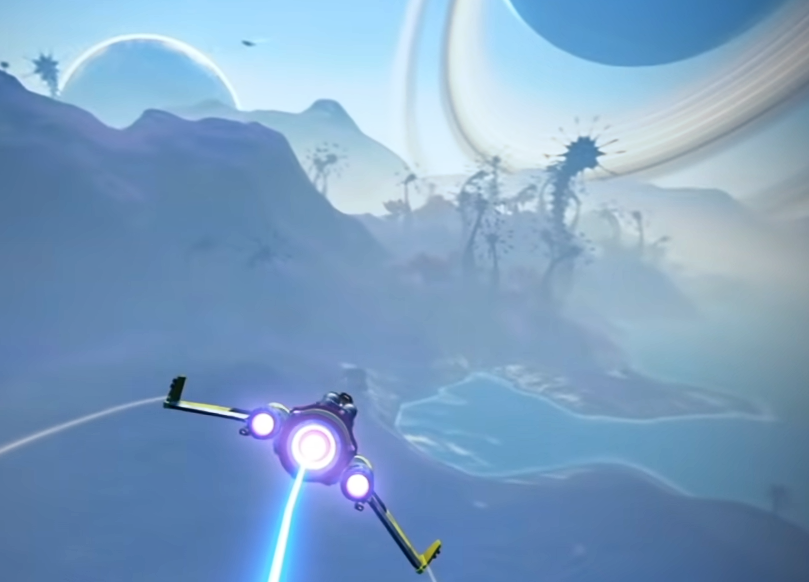
\includegraphics[height=0.8\textheight]{image/nomanssky}
    
    \smallskip
    
    \footnotesize{Részlet a \textit{No Man's Sky Origins} játékból (hivatalos trailer)}
\end{frame}

\section{A HoloDB felépítése}
\def\sectionshorttitle{\arabic{section}. Felépítés}

\begin{frame}
    \slidetitle{\sectionshorttitle}{Elvárások az új megoldással szemben}
    
    \begin{itemize}
        \setlength\itemsep{0.5em}
        \item {\color{red}relációs adatmodell}re épül
        \item {\color{red}deklaratív}, finomhangolható, könnyen bővíthető
        \item {\color{red}nincs preparálás}i folyamat, szinte azonnal elindul
        \item óriás adatmennyiséget is képes szimulálni, szinte {\color{red}tárhelyigény nélkül}
        \item az adatokat csak elérésükkor, on-the-fly számítja
        \item indexelt, a runtime teljesítmény elfogadható
        \item determinisztikus, {\color{red}koherens}, skálázható
        \item opcionálisan írható
    \end{itemize}
\end{frame}

\begin{frame}[fragile]
    \slidetitle{\sectionshorttitle}{Konfiguráció-példa}
    
    \centering
    
    \begin{minipage}[c]{0.47\textwidth}
        \centering
        
        \begin{minted}[
            fontsize=\tiny,
            framesep=4pt,
            frame=single,
            framerule=1.5pt,
            rulecolor=\color{gray!30}
        ]{yaml}
seed: 425364
schemas:
  - name: shop
    tables:
      - name: customers
        size: 5
        columns:
          - name: id
            mode: COUNTER
          - name: firstname
            valuesBundle: forenames
          - name: lastname
            valuesBundle: surnames
          - name: birth
            valuesRange: [1950, 2000]
      - name: orders
        size: 12
        columns:
          - name: id
            mode: COUNTER
          - name: cid
            valuesForeignColumn: [customers, id]
          - name: product
            valuesBundle: fruits
          - name: quantity
            valuesRange: [1, 10]
        \end{minted}
        
        {\footnotesize\texttt{config.yaml}} \pause
    \end{minipage}%
    \hspace*{\fill}
    \begin{minipage}[c]{0.35cm}
        {\Large $\Rightarrow$}
    \end{minipage}%
    \hspace*{\fill}
    \begin{minipage}[c]{0.45\textwidth}
        
        \centering
        
        \normalsize \texttt{customers}
        \vspace{0.1cm}
        
        \tiny
        \begin{tabular}{ |r|l|l|r| }
        \hline
           id & firstname & lastname & birth \\
        \hline
            1 & Howard & Anderson & 1968 \\
            2 & Rebecca & Ferguson & 1959 \\
            3 & Jeremy & Moore & 2000 \\
            4 & Julie & Ellis & 1951 \\
            5 & Kathleen & Cook & 1971 \\
        \hline
        \end{tabular}
        
        \vspace{0.5cm}
        
        \normalsize \texttt{orders}
        \vspace{0.1cm}
        
        \tiny
        \begin{tabular}{ |r|r|l|r| }
        \hline
            id & cid & ~~product & quantity \\
        \hline
            1 & 5 & date & 10 \\
            2 & 2 & orange & 1 \\
            3 & 2 & sloe & 2 \\
            4 & 3 & melon & 7 \\
            5 & 5 & guava & 9 \\
            6 & 3 & orange & 6 \\
            7 & 2 & plantain & 3 \\
            8 & 4 & pear & 7 \\
            9 & 4 & papaya & 9 \\
            10 & 5 & lime & 9 \\
            11 & 3 & sloe & 4 \\
            12 & 1 & strawberry & 1 \\
        \hline
        \end{tabular}
    \end{minipage}
\end{frame}

\begin{frame}
    \slidetitle{\sectionshorttitle}{Az architektúra áttekintése}
    
    \centering
    
    \begin{minipage}[c]{0.4\textwidth}
        \begin{overprint}
            \onslide<1>\centerline{\includegraphics[width=\textwidth]{diagram/simplearch-0}}
            \onslide<2-3>\centerline{\includegraphics[width=\textwidth]{diagram/simplearch-1}}
        \end{overprint}
    \end{minipage}%
    \hspace*{\fill}
    \begin{minipage}[c]{0.29\textwidth}
        \begin{overprint}
            \onslide<2-3>\begin{itemize}
                \item \texttt{Schema}
                \item \texttt{Table}
                \item \texttt{Column}
                \item \texttt{ColumnDefinition}
                \item {\only<3>{\color{beamer@blendedblue}\underline}{\texttt{Source}}}
                \item \texttt{Row}
                \item \texttt{TableIndex}
                \item \texttt{FulltextIndex}
                \item \texttt{SpatialIndex}
                \item \texttt{TableSelection}
            \end{itemize}
        \end{overprint}
    \end{minipage}%
    \begin{minipage}[c]{0.29\textwidth}
        \begin{overprint}
            \onslide<3>\centerline{\includegraphics[width=\textwidth]{diagram/storage-source}}
        \end{overprint}
    \end{minipage}%
    \hspace*{\fill}%
\end{frame}

\begin{frame}
    \slidetitle{\sectionshorttitle}{Alapvető adattípus: LargeInteger}
    
    \begin{minipage}[t]{0.6\textwidth}
        \centering
        
        \vspace{0.5em}
        
        \begin{itemize}
            \setlength\itemsep{0.5em}
            \item kis és óriás egészekkel is működik
            \item a konverzió automatikus és egyértelmű
            \item kis számokon gyors (\texttt{long} aritmetika)
            \item memóriaigénye minimális
            \item duplikálja a \texttt{BigInteger} metódusait
            \item további hasznos metódusokkal bővíti
            \item nincsenek függőségei
        \end{itemize}
    \end{minipage}%
    \begin{minipage}[t]{0.4\textwidth}
        \centering
        
        \vspace{0.05em}
        
        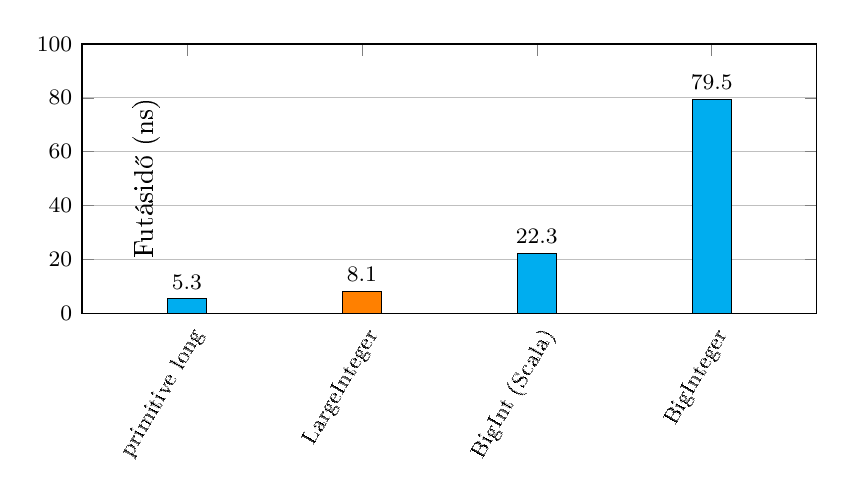
\begin{tikzpicture}[font=\footnotesize]
            \begin{axis}[
                    symbolic x coords={primitive long,,LargeInteger,,BigInt (Scala),,BigInteger},
                    xticklabel style={rotate=60,anchor=north east},
                    xtick={primitive long,LargeInteger,BigInt (Scala),BigInteger},
                    ylabel={Futásidő (ns)},
                    y label style={at={(0.12,0.5)}},
                    width={0.9\textwidth},
                    height=5cm,
                    ymajorgrids,
                    ymin=0,
                    ymax=100,
                    bar width=0.5cm,
                    enlarge x limits=0.2,
                    nodes near coords,
                    nodes near coords align={vertical},
                ]
                \addplot[ybar,fill=cyan] coordinates { (primitive long,5.3) };
                \addplot[ybar,fill=orange] coordinates { (LargeInteger,8.1) };
                \addplot[ybar,fill=cyan] coordinates { (BigInt (Scala),22.3) };
                \addplot[ybar,fill=cyan] coordinates { (BigInteger,79.5) };
            \end{axis}
        \end{tikzpicture}
    \end{minipage}
    
    \begin{flushright}
        { \footnotesize Benchmark: kis számokon végzett sokféle művelet ~~~~~ }
    \end{flushright}
\end{frame}

\begin{frame}
    \slidetitle{\sectionshorttitle}{Alapvető adattípus: TreeRandom}
    
    \begin{minipage}[c]{0.5\textwidth}
        \vspace{0.5em}
        
        {\color{beamer@blendedblue}Hierarchikus véletlengenerátor}
        
        \vspace{0.2cm}
        
        \begin{itemize}
            \item kulcs megadásával alpéldány
            \item egyenlő kulcs $\to$ egyenlő alpéldány
            \item egyenlő példány $\to$ egyező kimenet
        \end{itemize}

        \vspace{0.7cm}
        
        {\color{beamer@blendedblue}Gyenge követelmények}

        \vspace{0.2cm}
        
        \begin{itemize}
            \item véletlenszerű kimenetet ad
            \item eltérő példány $\to$ eltérő kimenet
        \end{itemize}

        \begin{overprint}
            \onslide<6>\begin{flushright}
                \vspace{2.5em}
                
                { \tiny \color{BrickRed}
                    \texttt{871121}{\color{RoyalPurple},}%
                    \texttt{"schema1"}{\color{RoyalPurple},}%
                    \texttt{"table1"}{\color{RoyalPurple},}%
                    \texttt{"description"}{\color{RoyalPurple},}%
                    \texttt{3}{\color{RoyalPurple},}%
                    \texttt{"text"} {\color{RoyalPurple}$\rightarrow$}
                    seed
                }
            \end{flushright}
        \end{overprint}
    \end{minipage}%
    \begin{minipage}[c]{0.5\textwidth}
        \begin{overprint}
            \onslide<2>\centerline{\includegraphics[height=0.85\textheight]{diagram/treerandom-0}}
            \onslide<3>\centerline{\includegraphics[height=0.85\textheight]{diagram/treerandom-1}}
            \onslide<4>\centerline{\includegraphics[height=0.85\textheight]{diagram/treerandom}}
            \onslide<5-6>\centerline{\includegraphics[height=0.85\textheight]{diagram/treerandom-nonindexed}}
            \onslide<7>\centerline{\includegraphics[height=0.85\textheight]{diagram/treerandom-indexed}}
        \end{overprint}
    \end{minipage}
\end{frame}

\begin{frame}[t,fragile]
    \slidetitle{\sectionshorttitle}{Alapvető adattípus: Permutation}
    
    \vspace{0.3em}
    
    \begin{minipage}[t]{0.33\textwidth}
        \vspace{0.5em}
        
        {\color{beamer@blendedblue}Követelmények permutációkra:}

        \vspace{0.2cm}
        
        \begin{itemize}
            \item $\mathbb{N} \to \mathbb{N}$ (\texttt{LargeInteger})
            \item véletlen-elérésű
            \item tetszőleges méretű
            \item hatékony inverz
            \item látszólag véletlenszerű
            \item kulccsal keverhető
        \end{itemize}
    \end{minipage}%
    \begin{minipage}[t]{0.65\textwidth}
        \centering
        
        {\footnotesize
        \begin{tabular}[t]{|l||r|r|r|r|} 
        \hline
        ~
            & \begin{tabular}{c} \textbftt{mem} \\ (bytes) \end{tabular}
            & \begin{tabular}{c} \textbftt{paq8/4} \\ (\%) \end{tabular}
            & \begin{tabular}{c} \textbftt{create} \\ (ns) \end{tabular}
            & \begin{tabular}{c} \textbftt{at×30} \\ (ns) \end{tabular}\\
        \hline\hline
        \textbftt{FAV} & 648 & 31,54 & 968 &  2~040 \\
        \hline
        \textbftt{MP1} & \best{152} & \bad{0,19} & \best{267} & \best{161} \\
        \hline
        \textbftt{FEI-F-4} & 608 & 19,56 & 660 & 8~800 \\
        \hline
        \textbftt{FEI-S-2} & \bad{212~312} & 97,08 & 434 & \bad{32~221} \\
        \hline
        \textbftt{FPE1} & \bad{211~352} & \best{97,07} & 540 & \bad{67~155} \\
        \hline
        \end{tabular}
        }
        
        \vspace{1.5em}
        
        \begin{minipage}[b]{0.25\textwidth}
            \centering
            
\includegraphics[width=0.97\textwidth]{image/permutation-fav.png}
            \par FAV
        \end{minipage}%
        \begin{minipage}[b]{0.25\textwidth}
            \centering
            
\includegraphics[width=0.97\textwidth]{image/permutation-mp1.png}
             \par MP1
        \end{minipage}%
        \begin{minipage}[b]{0.25\textwidth}
            \centering
            
\includegraphics[width=0.97\textwidth]{image/permutation-feif4.png}
            \par FEI-F-4
        \end{minipage}%
        \begin{minipage}[b]{0.25\textwidth}
            \centering
            
\includegraphics[width=0.97\textwidth]{image/permutation-feis2.png}
            \par FEI-S-2
        \end{minipage}%
        
    \end{minipage}
    
\end{frame}

\begin{frame}
    \slidetitle{\sectionshorttitle}{Általános kétlépéses értékkiosztás}
    
    \centering
    
    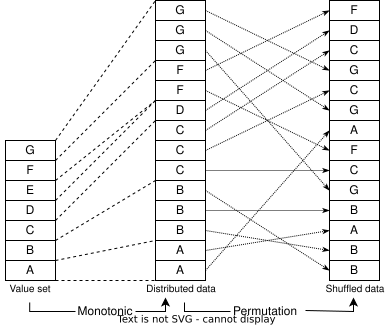
\includegraphics[height=0.7\textheight]{diagram/distribution}
    
    A kétlépéses értékkiosztás alapelve: \par
    visszafejthető disztribúció és permutáció kompozíciója
\end{frame}

\begin{frame}
    \slidetitle{\sectionshorttitle}{Írhatósági réteg}
    
    \begin{minipage}[c]{0.65\textwidth}
        {\color{beamer@blendedblue}A \texttt{DiffTable} dekorátor}
        
        \begin{itemize}
            \item csak olvassa az alárendelt táblaobjektumot
            \item amíg nincs módosítás, átlátszóan működik
            \item memóriában tárolja a módosításokat
            \item átírhatja a lekérést és összefésülheti az eredménytáblát
        \end{itemize}
        
        \vspace{0.4cm}
        
        {\color{beamer@blendedblue}Tranzakciókezelés}
        
        \begin{itemize}
            \item kétféle tranzakciós stratégia: írási ablakok vagy MVCC
            \item kétféle commit mód: \texttt{AUTOCOMMIT} vagy explicit lockolás
            \item mindegyik változat ACID-kompatibilis
            \item nagyon sok írási művelet esetén nem igazán hatékony
        \end{itemize}
    \end{minipage}%
    \hspace*{\fill}%
    \begin{minipage}[c]{0.32\textwidth}
        \centering
        
        \includegraphics[height=0.8\textheight]{diagram/distribution-write}
    \end{minipage}%
    \hspace*{\fill}%
\end{frame}

\begin{frame}
    \slidetitle{\sectionshorttitle}{Kétlépéses értékkiosztás: adatlekérés}
    
    \centering
    
    \begin{overprint}
        \onslide<1>\centerline{\includegraphics[height=0.7\textheight]{diagram/getvalue-0}}
        \onslide<2>\centerline{\includegraphics[height=0.7\textheight]{diagram/getvalue-1}}
        \onslide<3>\centerline{\includegraphics[height=0.7\textheight]{diagram/getvalue-2}}
        \onslide<4>\centerline{\includegraphics[height=0.7\textheight]{diagram/getvalue-3}}
        \onslide<5>\centerline{\includegraphics[height=0.7\textheight]{diagram/getvalue-4}}
        \onslide<6->\centerline{\includegraphics[height=0.7\textheight]{diagram/getvalue-5}}
    \end{overprint}
    
    \hspace{0.7cm}
    
    Lekövetjük, melyik érték képződik a virtuális értéklista adott pozíciójára
\end{frame}

\begin{frame}
    \slidetitle{\sectionshorttitle}{Kétlépéses értékkiosztás: keresés}
    
    \centering
    
    \begin{overprint}
        \onslide<1>\centerline{\includegraphics[height=0.7\textheight]{diagram/findvalue-0}}
        \onslide<2>\centerline{\includegraphics[height=0.7\textheight]{diagram/findvalue-1}}
        \onslide<3>\centerline{\includegraphics[height=0.7\textheight]{diagram/findvalue-2}}
        \onslide<4->\centerline{\includegraphics[height=0.7\textheight]{diagram/findvalue-3}}
    \end{overprint}
    
    \vspace{0.7cm}
    
    Eset: az érték szerepel az oszlop virtuális értéklistájában
\end{frame}

\begin{frame}
    \slidetitle{\sectionshorttitle}{Kétlépéses értékkiosztás: nincs találat}
    
    \centering
    
    \includegraphics[height=0.7\textheight]{diagram/findvalue2-merged}
    
    \vspace{0.7cm}
    
    Eset: az érték nem található, mert nincs az értékkészletben vagy nincs kiosztva
\end{frame}

\begin{frame}
    \slidetitle{\sectionshorttitle}{Kétlépéses értékkiosztás: értéksáv keresése}
    
    \centering
    
    \includegraphics[height=0.7\textheight]{diagram/findvaluerange}
    
    \vspace{0.7cm}
    
    Eset: keresés értéksávra; a hiányzó határoló érték pozíciója is fontos
\end{frame}

\begin{frame}[t]
    \slidetitle{\sectionshorttitle}{Értékek reguláris kifejezésből, kereshetően}
    \centering
    {\Large A \texttt{\colorbox{Goldenrod!10}{([a-c]z(tt|uu)r|a[x-z])}} reguláris kifejezés {\color{red}nyers} szófája:}
    
    \vspace{1.2cm}
    
    \includesvg[width=\textwidth]{diagram/trie-simple-raw}
\end{frame}

\begin{frame}[t,noframenumbering]
    \slidetitle{\sectionshorttitle}{Értékek reguláris kifejezésből, kereshetően}
    \centering
    {\Large A \texttt{\colorbox{Goldenrod!10}{([a-c]z(tt|uu)r|a[x-z])}} reguláris kifejezés {\color{red}kompakt} szófája:}
    
    \vspace{1.2cm}
    
    \includesvg[width=\textwidth]{diagram/trie-simple-compact}
\end{frame}

\section{Tapasztalatok, mérési eredmények}
\def\sectionshorttitle{\arabic{section}. Tapasztalatok}

\begin{frame}[fragile]
    \slidetitle{\sectionshorttitle}{Lekérdezések sebessége}
    
    \centering
    
    \begin{tabular}{|l||r|r|r|r|r||} 
    \hline
    ~
        & \begin{tabular}{c} \textbftt{Q-FLD} \\ ({\textmu}s) \end{tabular}
        & \begin{tabular}{c} \textbftt{Q-REC} \\ ({\textmu}s) \end{tabular}
        & \begin{tabular}{c} \textbftt{Q-TFUL} \\ ({\textmu}s) \end{tabular}
        & \begin{tabular}{c} \textbftt{Q-MULT} \\ ({\textmu}s) \end{tabular}\\
    \hline\hline

    \textbf{HoloDB/}\textbftt{EXT} & 43,00 & 180,35 & \bad{1~514~177} & \bad{6~818} \\
    \textbf{HoloDB/}\textbftt{DEF} & 24,66 & 130,08 & \bad{1~143~721} & \bad{3~592} \\
    \textbf{HoloDB/}\textbftt{MIN} & 22,82 & 20,22 & 25~909 & 365 \\
    \textbf{H2}& \best{12,77} & \best{9,73} & \best{1~965} & \best{177} \\
    \textbf{MariaDB} & 47,87 & 46,27 & 3~393 & 1~429 \\
    \hline
    \end{tabular}
    
    \vspace{0.5em}
    
    Lekérdezési tesztek eredménye különböző adatbázisokkal.
    
    \vspace{1.5em}
    
    \hspace*{\fill}%
    \begin{minipage}[t]{0.52\textwidth}
        \makebox[3.3em][l]{\small{\textbftt{Q-FLD}:}}
        {\scriptsize{\mintinline{sql}{SELECT firstname FROM students WHERE id=30}}}
        
        \vspace{0.7em}
        
        \makebox[3.3em][l]{\small{\textbftt{Q-REC}:}}
        {\scriptsize{\mintinline{sql}{SELECT * FROM students WHERE id=30}}}
        
        \vspace{0.7em}
        
        \makebox[3.3em][l]{\small{\textbftt{Q-TFUL}:}}
        {\scriptsize{\mintinline{sql}{SELECT * FROM students}}}
    \end{minipage}
    \hspace*{\fill}%
    \begin{minipage}[t]{0.45\textwidth}
        {\small{\textbftt{Q-MULT}:}}
        
        \vspace{-2em}
        \hspace{1em}%
        \begin{minted}[
            fontsize=\scriptsize,
            frame=none,
            bgcolor=white,
            baselinestretch=1,
            linenos=false,
        ]{sql}
SELECT s.lastname FROM students s
LEFT JOIN course_student cs ON cs.sid=s.id
LEFT JOIN courses c ON c.id=cs.cid
LEFT JOIN subjects su ON su.id=c.sid
WHERE s.firstname='Ian' AND su.id=2
        \end{minted}
    \end{minipage}
    \hspace*{\fill}%
\end{frame}

\begin{frame}
    \slidetitle{\sectionshorttitle}{Integrált teszt webes alkalmazással}
    
    \centering
    
    \begin{tabular}{|l||r|r|r||} 
    \hline
    ~
        & \begin{tabular}{c} \textbftt{RO-SIMP} \\ (s) \end{tabular}
        & \begin{tabular}{c} \textbftt{RO-CMPX} \\ (s) \end{tabular}
        & \begin{tabular}{c} \textbftt{WR-CMPX} \\ (s) \end{tabular}\\
    \hline\hline
    
    \textbf{HoloDB/}\textbftt{EXT} & 6,79 & 7,10 & 12,16 \\
    \textbf{HoloDB/}\textbftt{DEF} & 6,36 & 6,56 & 11,09 \\
    \textbf{HoloDB/}\textbftt{MIN} & 4,60 & 4,76 &  7,54 \\
    \textbf{H2} & \best{3,92} & \best{4,02} &  \best{6,07} \\
    \textbf{MariaDB} & 5,10 & 5,43 &  8,38 \\
    \hline
    \end{tabular}
    
    \vspace{0.5em}
    
    Integrált tesztek eredménye különböző adatbázisokkal.
    
    
    \vspace{1em}
    
    \begin{minipage}[t]{0.75\textwidth}
        \textbftt{RO-SIMP}: egyszerű adatlekérdezések (10~203 hívás)
        
        \textbftt{RO-CMPX}: az előbbi teszt kiegészítve statisztikai lekérdezésekkel
        
        \textbftt{WR-CMPX}: az előbbi teszt kiegészítve írási műveletekkel
    \end{minipage}
\end{frame}

\begin{frame}
    \slidetitle{\sectionshorttitle}{Adathalmaz előállása}
    
    \centering
    
    \begin{tabular}{|l|l||r|r||r|r||}
    \hline
    ~
        & \textbf{Generátor}
        & \begin{tabular}{c} \textbf{Generálás} \\ (s) \end{tabular}
        & \begin{tabular}{c} \textbf{Indítás} \\ (s) \end{tabular}
        & \begin{tabular}{c} \textbf{Konfiguráció} \\ (B) \end{tabular}
        & \begin{tabular}{c} \textbf{Tárigény} \\ (MiB) \end{tabular}\\
    \hline\hline

    \textbf{HoloDB} & \nodata & \best{0,00} & \best{0,28} & \best{1~303} & \best{0,16} \\
    \textbf{MariaDB} & \textbf{Laravel seeder} & 7,08 & \best{0,28} & 7~944 & 0,45 \\
    \textbf{Postgres} & \textbf{SQL-szkript} & 0,20 & 2,25 & 2~005 & 1,40 \\
    \hline
    \end{tabular}
    
    \vspace{0.3em}
    
    Kisméretű adathalmaz (7~200 rekord) előállása különböző megoldásokkal.
    \pause
    
    \vspace{1.5em}
    
    \begin{tabular}{|l|l||r|r||r|r||} 
    \hline
    ~
        & \textbf{Generátor}
        & \begin{tabular}{c} \textbf{Generálás} \\ (s) \end{tabular}
        & \begin{tabular}{c} \textbf{Indítás} \\ (s) \end{tabular}
        & \begin{tabular}{c} \textbf{Konfiguráció} \\ (B) \end{tabular}
        & \begin{tabular}{c} \textbf{Tárigény} \\ (MiB) \end{tabular}\\
    \hline\hline
    \textbf{HoloDB} & \nodata & \best{0} & \best{0,28} & \best{1~311} & \best{0,16} \\
    \textbf{MariaDB} & \textbf{Laravel seeder} & \bad{15~734} & 0,30 & 8~008 & \bad{1~101,47} \\
    \textbf{Postgres} & \textbf{SQL-szkript} & 95 & 2,26 & 2~017 & \bad{1~409,57} \\
    \hline
    \end{tabular}
    
    \vspace{0.3em}
    
    Nagyméretű adathalmaz (11~002~000 rekord) előállása különböző megoldásokkal.
\end{frame}

\section{Összegzés}
\def\sectionshorttitle{\arabic{section}. Összegzés}

\begin{frame}
    \slidetitle{\sectionshorttitle}{Elvárások teljesítése}
%    
    \begin{itemize}
        \setlength\itemsep{0.5em}
        \item[\greencheck] {\color{red}relációs adatmodell}re épül
        \item[\greencheck] {\color{red}deklaratív}, finomhangolható, könnyen bővíthető
        \item[\greencheck] {\color{red}nincs preparálás}i folyamat, szinte azonnal elindul
        \item[\greencheck] óriás adatmennyiséget is képes szimulálni, szinte {\color{red}tárhelyigény nélkül}
        \item[\greencheck] az adatokat csak elérésükkor, on-the-fly számítja
        \item[\greencheck] indexelt, a runtime teljesítmény elfogadható
        \item[\greencheck] determinisztikus, {\color{red}koherens}, skálázható
        \item[\greencheck] opcionálisan írható
    \end{itemize}
\end{frame}

\begin{frame}
    \slidetitle{\sectionshorttitle}{További lehetőségek}
    
    \begin{itemize}
        \setlength\itemsep{1em}
        \item könnyen verziókezelhető
        \item könnyen replikálható (csak-olvasható adatbázis esetén)
        \item JPA-entitásokból is indítható (nem szükséges a YAML-fájl)
        \item füsttesztekhez is használható
        \item akár serverless szolgáltatásként is működtethető
        \item az írási réteg meglévő adatbázis fölé is elhelyezhető
        \item a konfiguráció újraindítás nélkül is újratölthető
    \end{itemize}
\end{frame}

\begin{frame}
    \slidetitle{\sectionshorttitle}{A közeljövő fő tervei}

    A meglévő funkciók továbbfejlesztésén, optimalizálásán túl:
    
    \vspace{1em}
    
    \hspace*{\fill}%
    \begin{minipage}[t]{0.7\textwidth}
        \begin{itemize}
            \setlength\itemsep{1em}
            \item további értékkészlet-típusok
            \item könnyen konfigurálható megkötések
            \item DBeaver-integráció
            \item általános keretrendszer letapogatáshoz és materializáláshoz
            \item HoloDB mint felhőszolgáltatás
            \item igényfelmérés, alkalmazás valós projekteken
        \end{itemize}
    \end{minipage}
    \hspace*{\fill}%
    \begin{minipage}[t]{0.29\textwidth}
        \vspace{1cm}
        
        \includesvg[width=\0.9\textwidth]{image/planning}
    \end{minipage}
    \hspace*{\fill}%
\end{frame}
        
\begin{frame}
    \vspace{1em}
    
    \centering
    
    { \Huge Köszönöm a figyelmet! }
    
    \vspace{3em}
    
    \hspace*{\fill}%
    \begin{minipage}[c]{0.75\textwidth}
        \begin{flushleft}
            \normalsize
            
            ~~~
            {\color{beamer@blendedblue}Linkek:}
            
            \vspace{0.5em}
            
            \footnotesize
            
            \begin{itemize}
                \item HoloDB projekt: \par
                    \url{https://github.com/miniconnect/holodb}
                \item Használati példák: \par
                    {\scriptsize{\url{https://github.com/miniconnect/general-docs/tree/main/examples}}}
                \item Jelen TDK-pályamunka forrásrepója: \par
                    \url{https://github.com/davidsusu/holodb-tdk}
            \end{itemize}
            
            \vspace{1.5em}
            
            \normalsize
            
            ~~~
            { \color{beamer@blendedblue} E-mail: }
            \href{mailto:horvathdown@student.elte.hu}{horvathdown@student.elte.hu}
        \end{flushleft}
    \end{minipage}%
    \hspace*{\fill}%
    \begin{minipage}[c]{0.24\textwidth}
        \scalebox{1.5}{\qrcode{https://github.com/miniconnect/holodb}}
    \end{minipage}%
    \hspace*{\fill}%
\end{frame}

\appendix
\begingroup
\setbeamertemplate{footline}{}

\section{Bírálói kérdések}
\def\sectionshorttitle{Kérdések}

\begin{frame}[c,noframenumbering]
    ~~~
    
    \brqr
\end{frame}

\begin{frame}[c,noframenumbering]
    \centering
    
    \Huge Bírálói kérdések
    
    \brqr
\end{frame}

\begin{frame}[t,noframenumbering]
    \slidetitle{\sectionshorttitle}{1. Több SQL dialektus}
    
    \textbf{%
    Tudna-e a rendszer támogatni különböző query nyelveket
    egy absztrakciós rétegen keresztül,
    hogy integrálni lehessen olyan rendszerekkel,
    amelyek kötve vannak egy bizonyos SQL típushoz?
    }
    
    \vspace{0.7cm}
    
    \begin{itemize}
        \setlength\itemsep{1em}
        \item \textbf{igen}
        \begin{itemize}
            \item a \texttt{QueryExecutor} implementációja cserélhető, jelenleg kétféle lehet:
            \begin{itemize}
                \item \texttt{default} (limitált SQL, gyors)
                \item Apache Calcite (kb. 40-féle dialektust támogat)
            \end{itemize}
            \item kezdetleges támogatás további lekérdezési módokhoz is elérhető:
            \begin{itemize}
                \item REST API
                \item GraphQL (GraphQL-Java)
                \item SPARQL (Quetzal)
            \end{itemize}
        \end{itemize}
    \end{itemize}
    
    \brqr
\end{frame}

\begin{frame}[t,noframenumbering,fragile]
    \slidetitle{\sectionshorttitle}{2. ORM-integráció}
    
    \textbf{%
    Lehetne-e integrációt nyújtani meglévő ORM keretrendszerekhez
    (pl. Hibernate)?
    Mennyire látja ezt megvalósíthatónak?
    }
    
    \vspace{0.3cm}
    
    \begin{itemize}
        \setlength\itemsep{1em}
        \item \textbf{támogatott}: konfiguráció helyett JPA entitások (opcionális kiegészítő annotációkkal):
    \end{itemize}
    
    \hspace*{0.05\textwidth}
    \begin{minipage}{0.72\textwidth}
        \begin{minted}[
            fontsize=\tiny,
            framesep=4pt,
            frame=single,
            framerule=1.5pt,
            rulecolor=\color{gray!30}
        ]{java}
@Entity
@Table(name = "posts")
@HoloTable(size = 500)
public class Post {
    @Id
    @GeneratedValue(strategy = GenerationType.IDENTITY)
    private Long id;
    
    @Column
    @HoloColumn(valuesBundle = "lorem")
    private String title;

    @Column(name = "tag")
    @ElementCollection
    @CollectionTable(name = "post_tags", joinColumns = { @JoinColumn(name = "post_id") })
    @HoloTable(size = 20)
    @HoloColumn(values = { "tag1", "tag2", "tag3" })
    @HoloVirtualColumn(name = "color", valuesBundle = "colors")
    private Set<String> tags;

    // ...
        \end{minted}
    \end{minipage}
    
    \brqr
\end{frame}

\begin{frame}[t,noframenumbering]
    \slidetitle{\sectionshorttitle}{3. Komplex megkötések}
    
    \textbf{%
    Tudna-e támogatni a megoldás egy tábla oszlopai közötti
    vagy akár különböző táblák közötti
    strukturális és komplex kényszereket?
    }
    
    \vspace{0.7cm}
    
    \begin{itemize}
        \setlength\itemsep{1em}
        \item jelenleg csak \textbf{részlegesen}
        \begin{itemize}
            \item konfigurációból jelenleg csak részhalmaz megkötések (pl. idegen kulcs) adhatók meg
            \item többoszlopos \texttt{Source} egyedileg hozzáadható
            \item más értékektől függő, nem indexelt \texttt{Source} egyedileg hozzáadható
        \end{itemize}
        \item minél több megkötés támogatása prioritás, már tervezés alatt:
        \begin{itemize}
            \item "kombinatorikus" virtuális index
            \item kényszerek könnyű konfigurálhatósága
        \end{itemize}
    \end{itemize}
    
    \brqr
\end{frame}

\endgroup

\end{document}
